\begin{figure*}[!t]
\centering
\subfloat[][Model size]{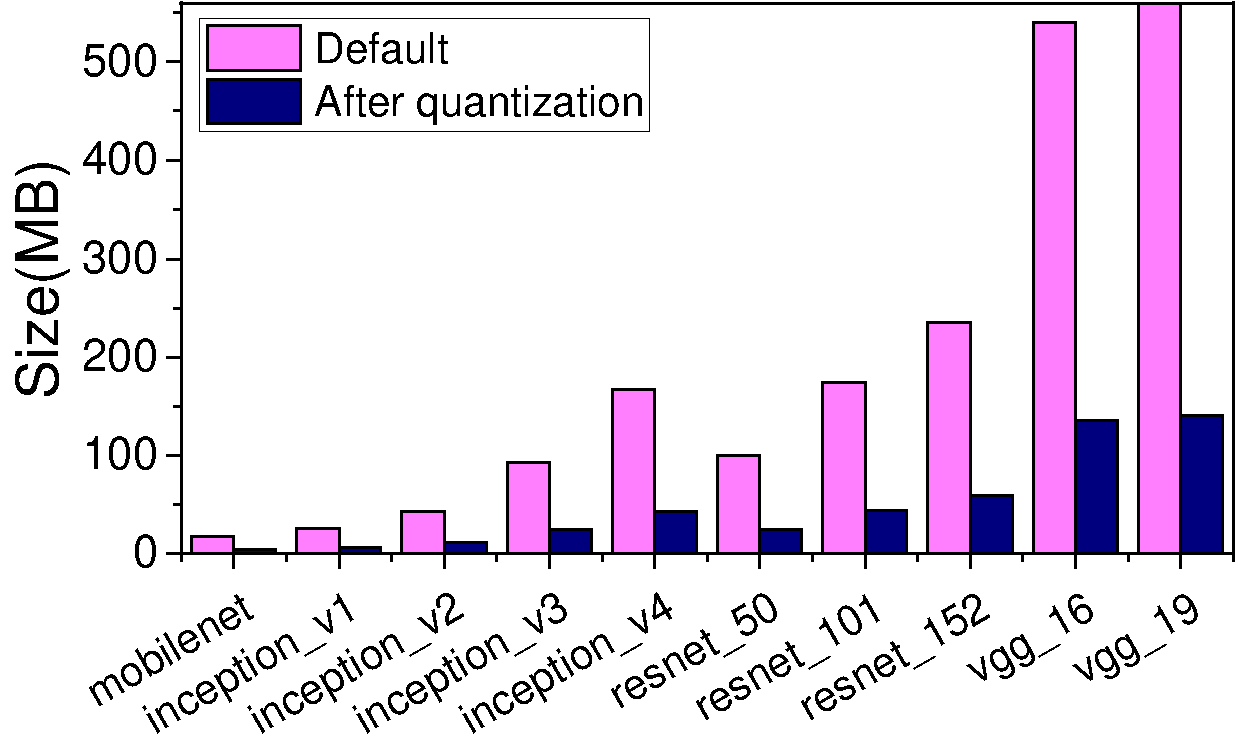
\includegraphics[width=0.33\textwidth]{figure/quan_size.pdf}}
\hfill
\subfloat[][Inference time]{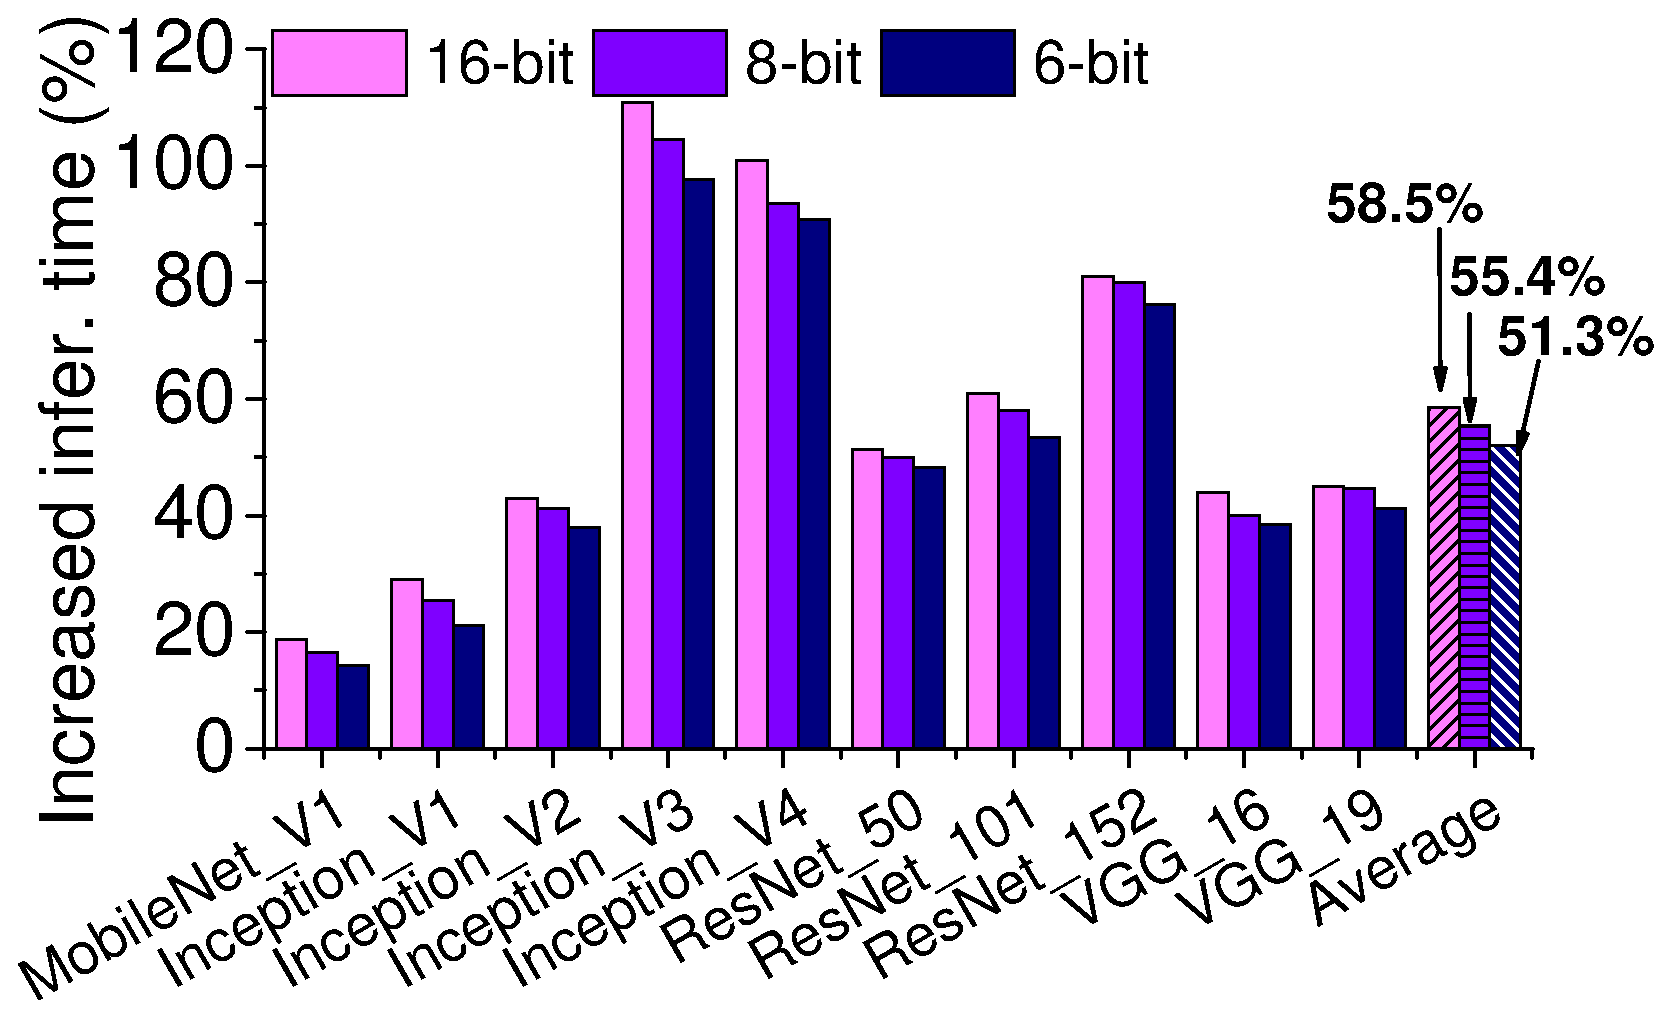
\includegraphics[width=0.34\textwidth]{figure/quan_time2.pdf}}
\hfill
\subfloat[][Accuracy]{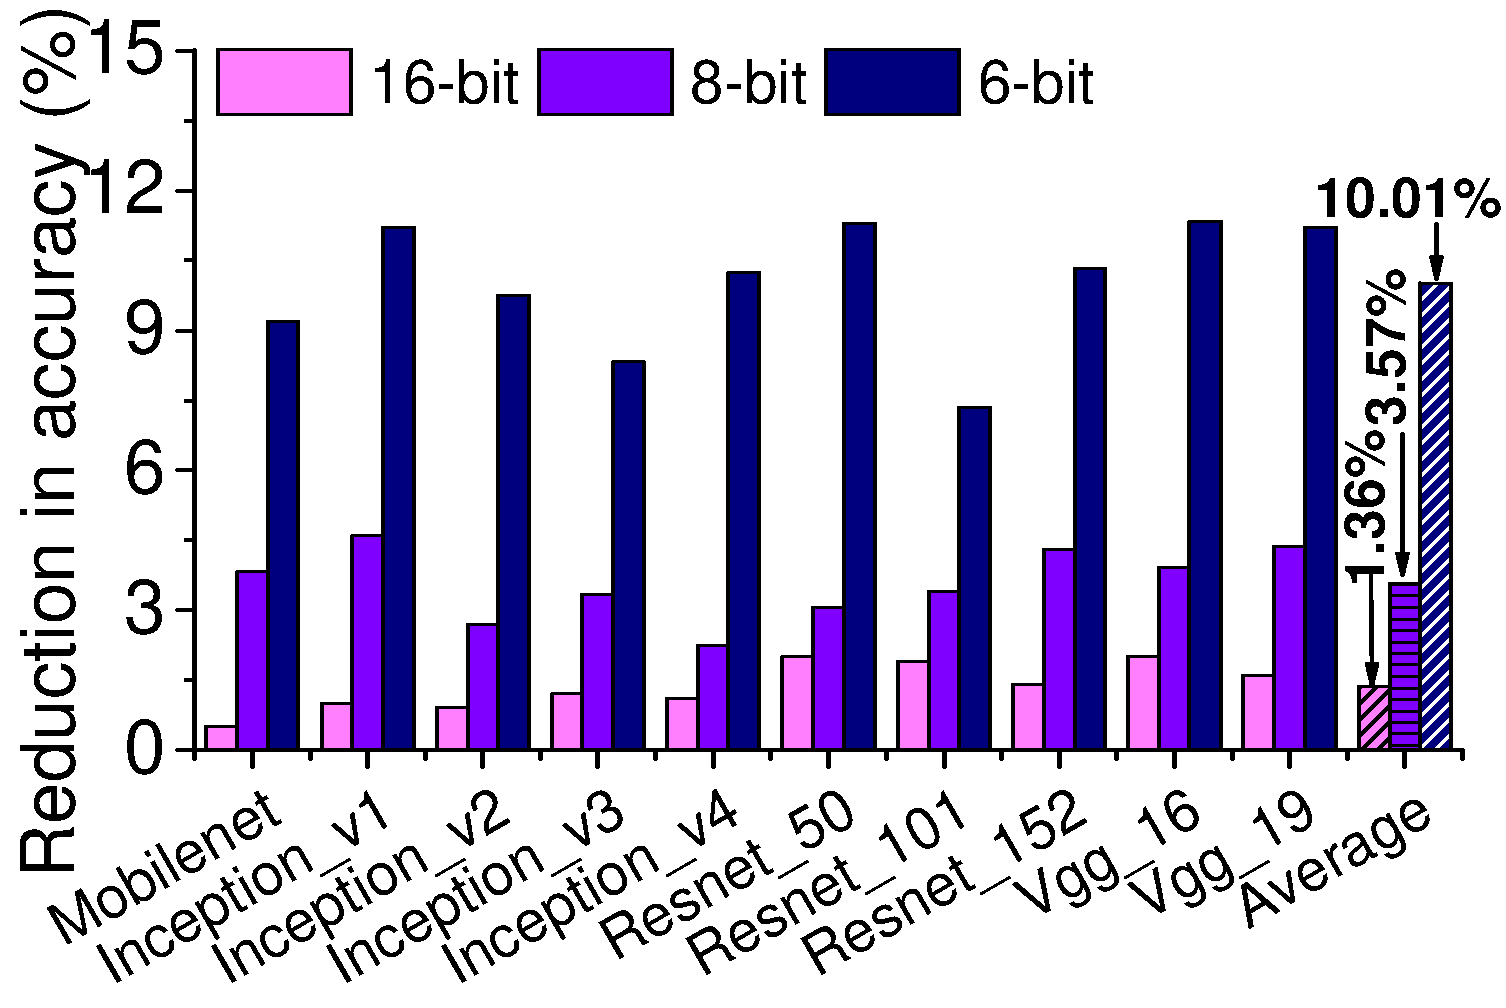
\includegraphics[width=0.32\textwidth]{figure/quan_acc3.pdf}}
\hfill
\subfloat[][Power consumption]{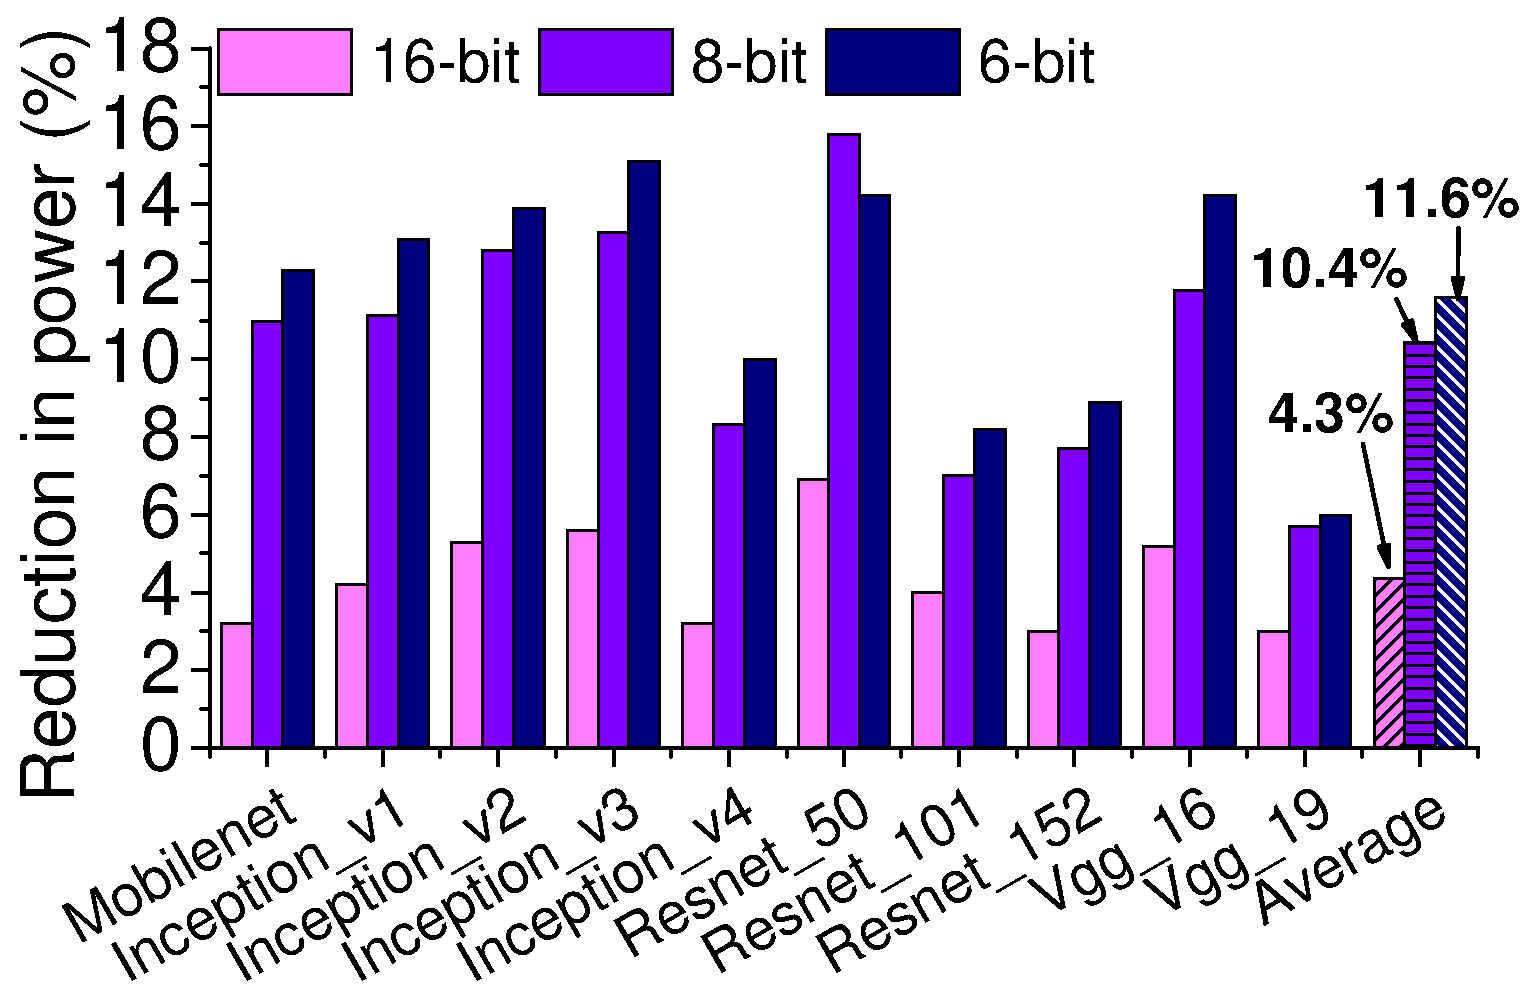
\includegraphics[width=0.33\textwidth]{figure/quan_power2.pdf}}
\hfill
\subfloat[][Energy consumption]{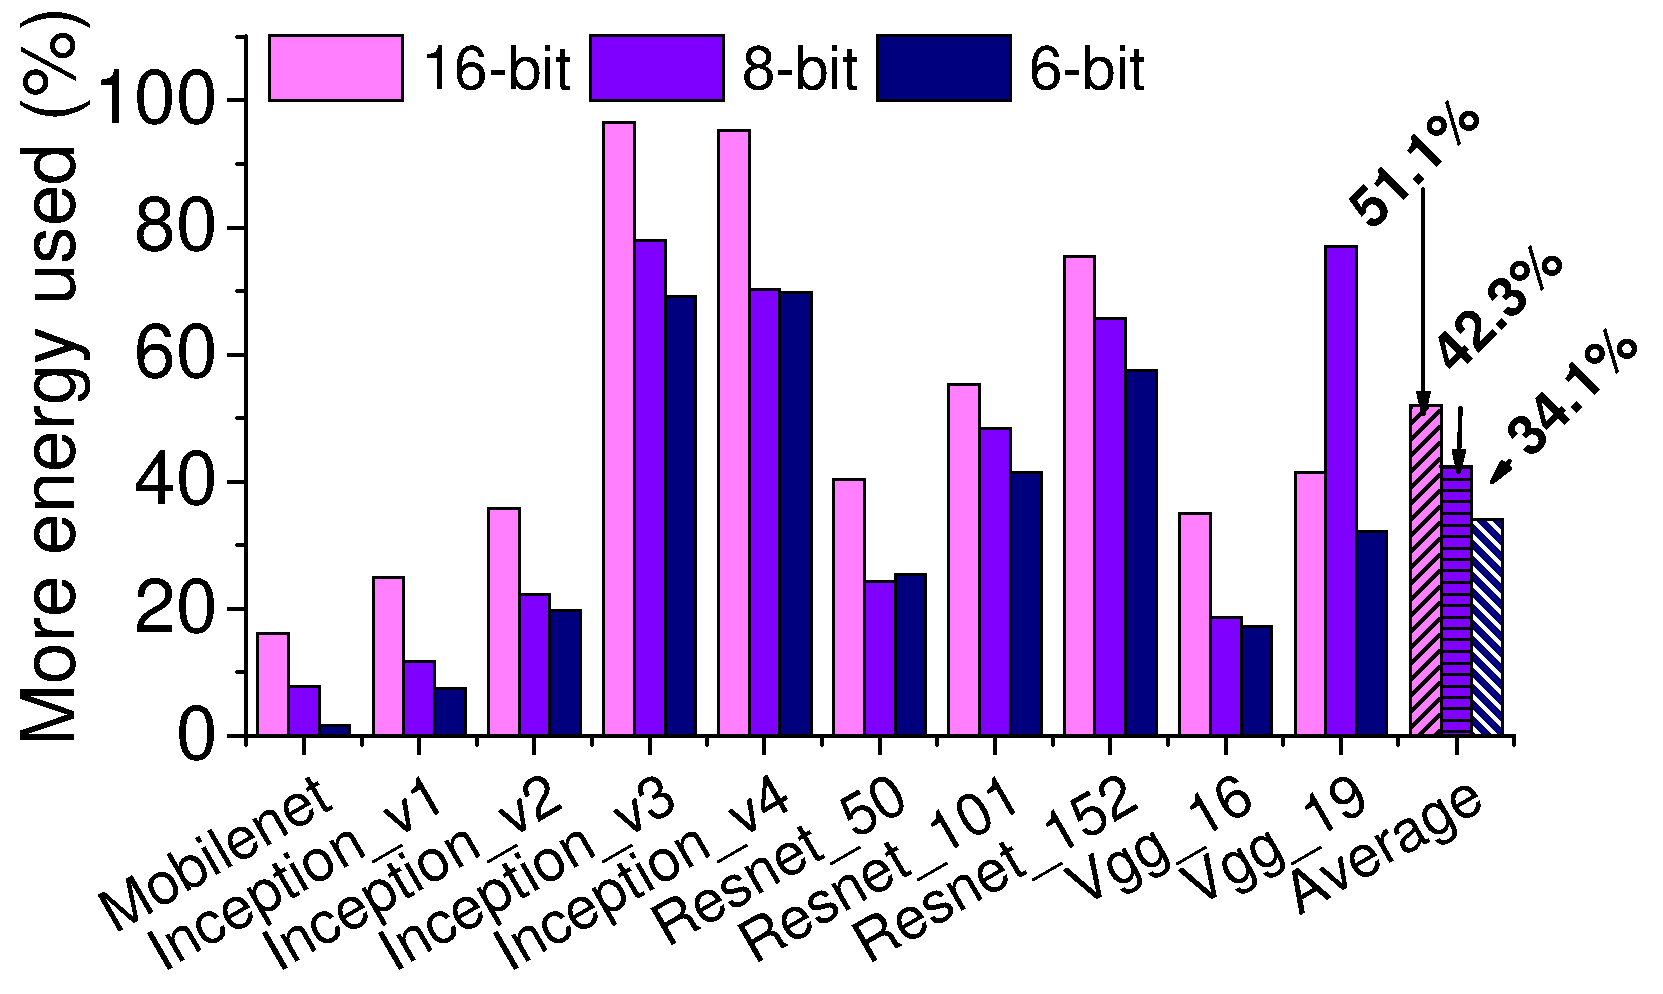
\includegraphics[width=0.34\textwidth]{figure/quan_energy2.pdf}}
\hfill
\subfloat[][precision, recall and F1 score]{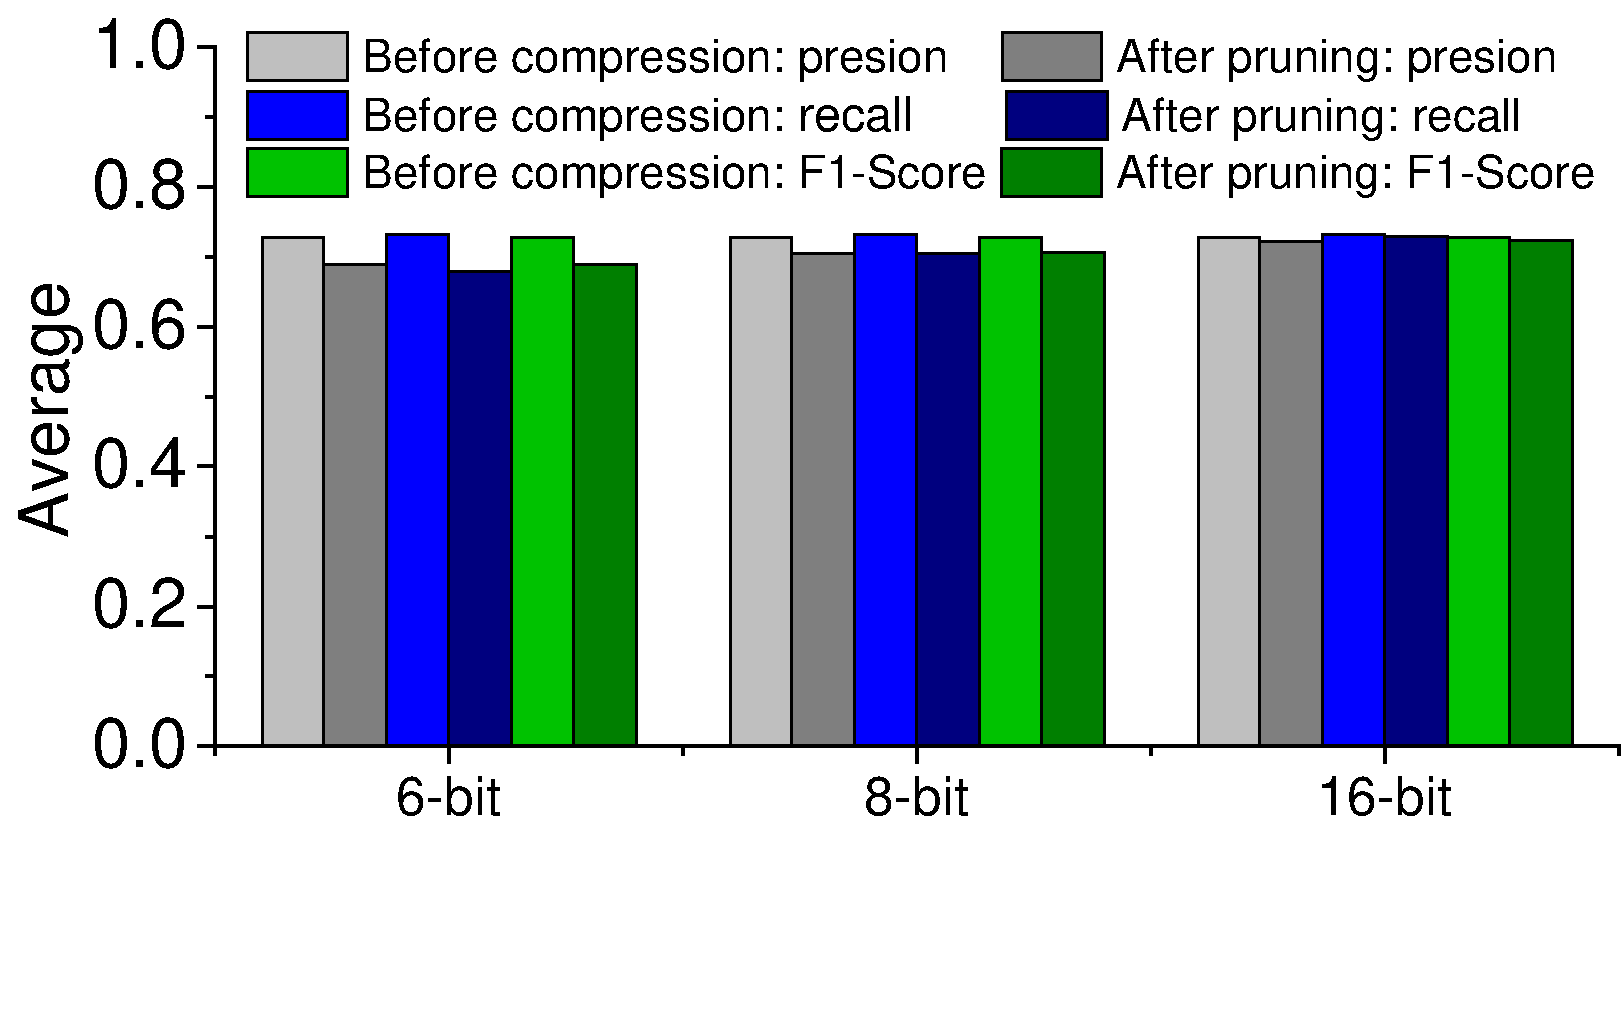
\includegraphics[width=0.33\textwidth]{figure/quan_prf2.pdf}}
\hfill

\caption{The achieved model size (a) inference time (b) accuracy (c) power consumption (d)
energy consumption (e) and precision, recall and F1 score (e) before and after the compression by \quantization.
The compression technique to use depends on the optimization target.}
\label{fig:analy_quan}
\end{figure*}


\begin{figure*}[!t]
\centering
\subfloat[][Model size]{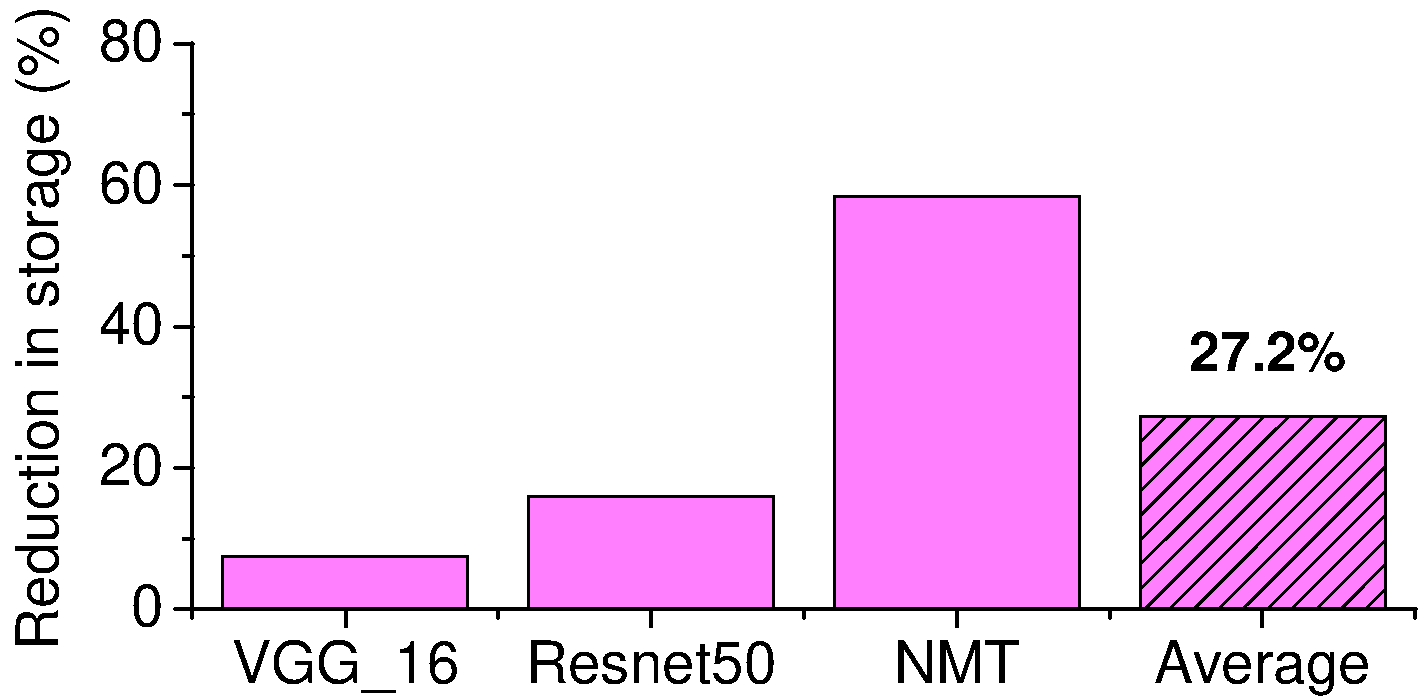
\includegraphics[width=0.33\textwidth]{figure/prun_size.pdf}}
\hfill
\subfloat[][Inference time]{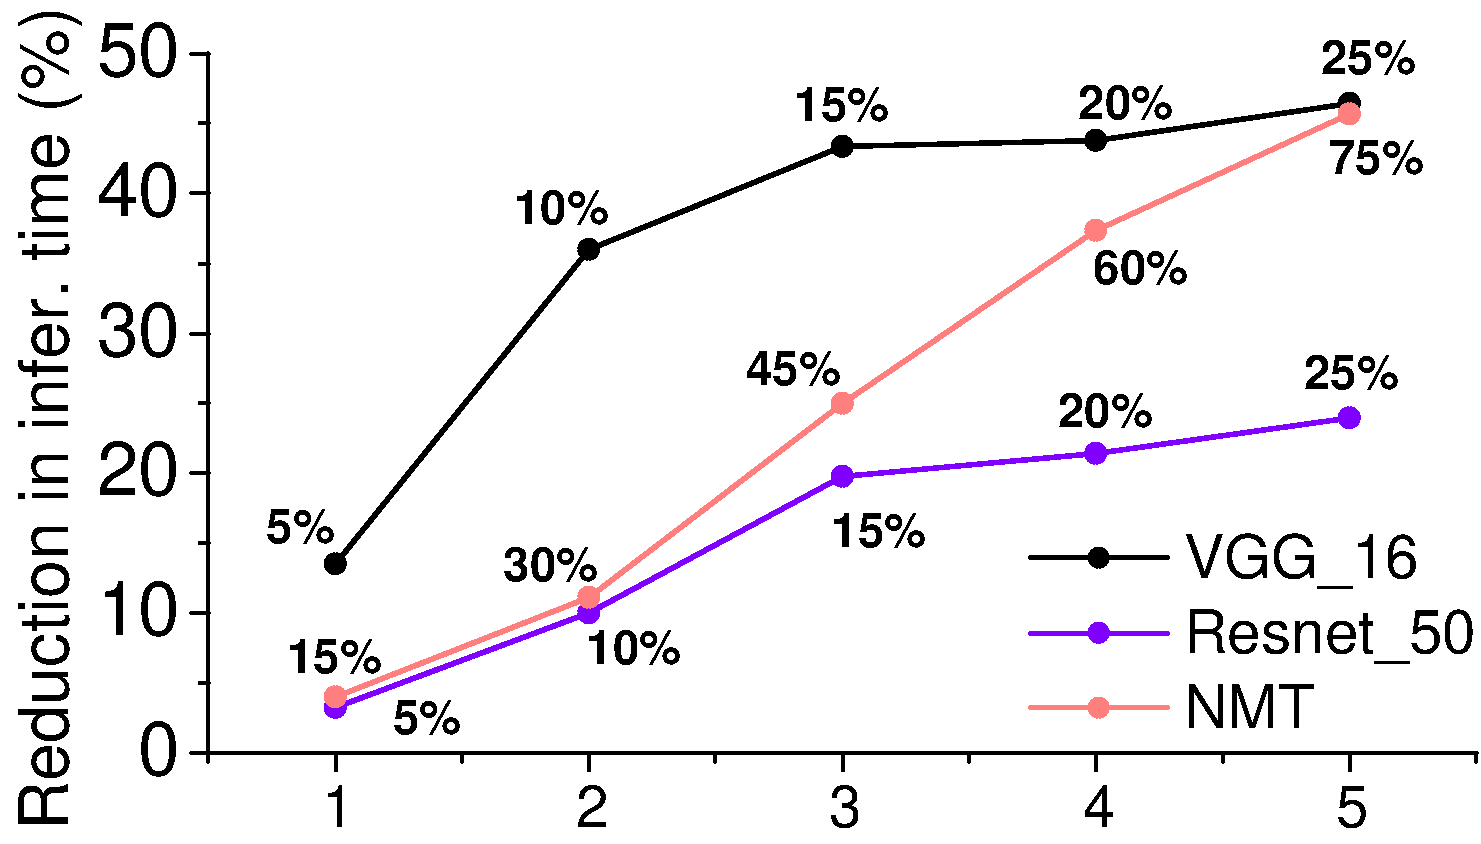
\includegraphics[width=0.3\textwidth]{figure/prun_time1.pdf}}
\hfill
\subfloat[][Accuracy]{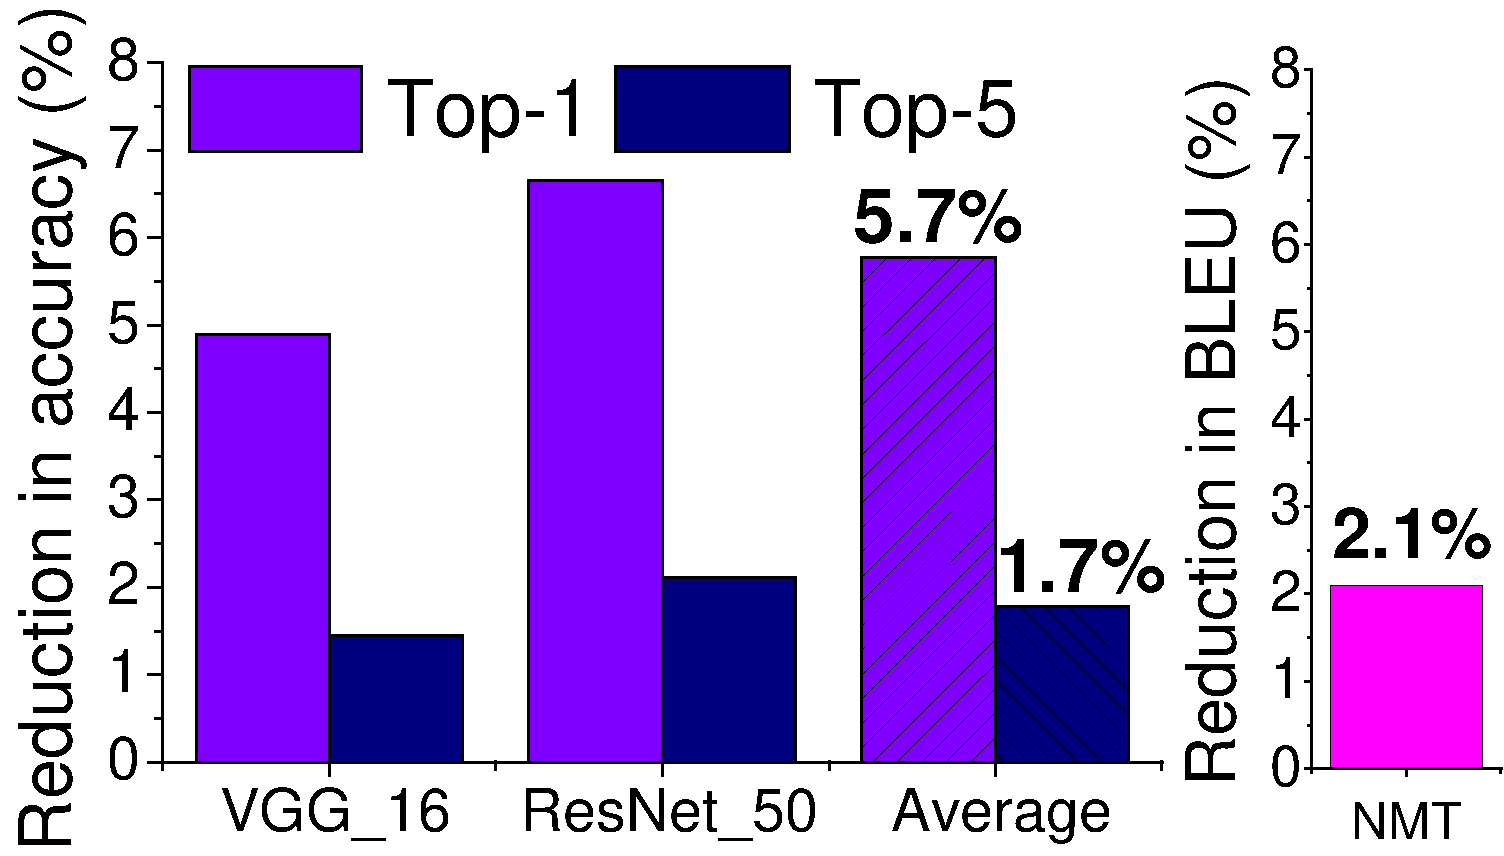
\includegraphics[width=0.3\textwidth]{figure/top1_5_prun.pdf}}
\hfill
\subfloat[][Power consumption]{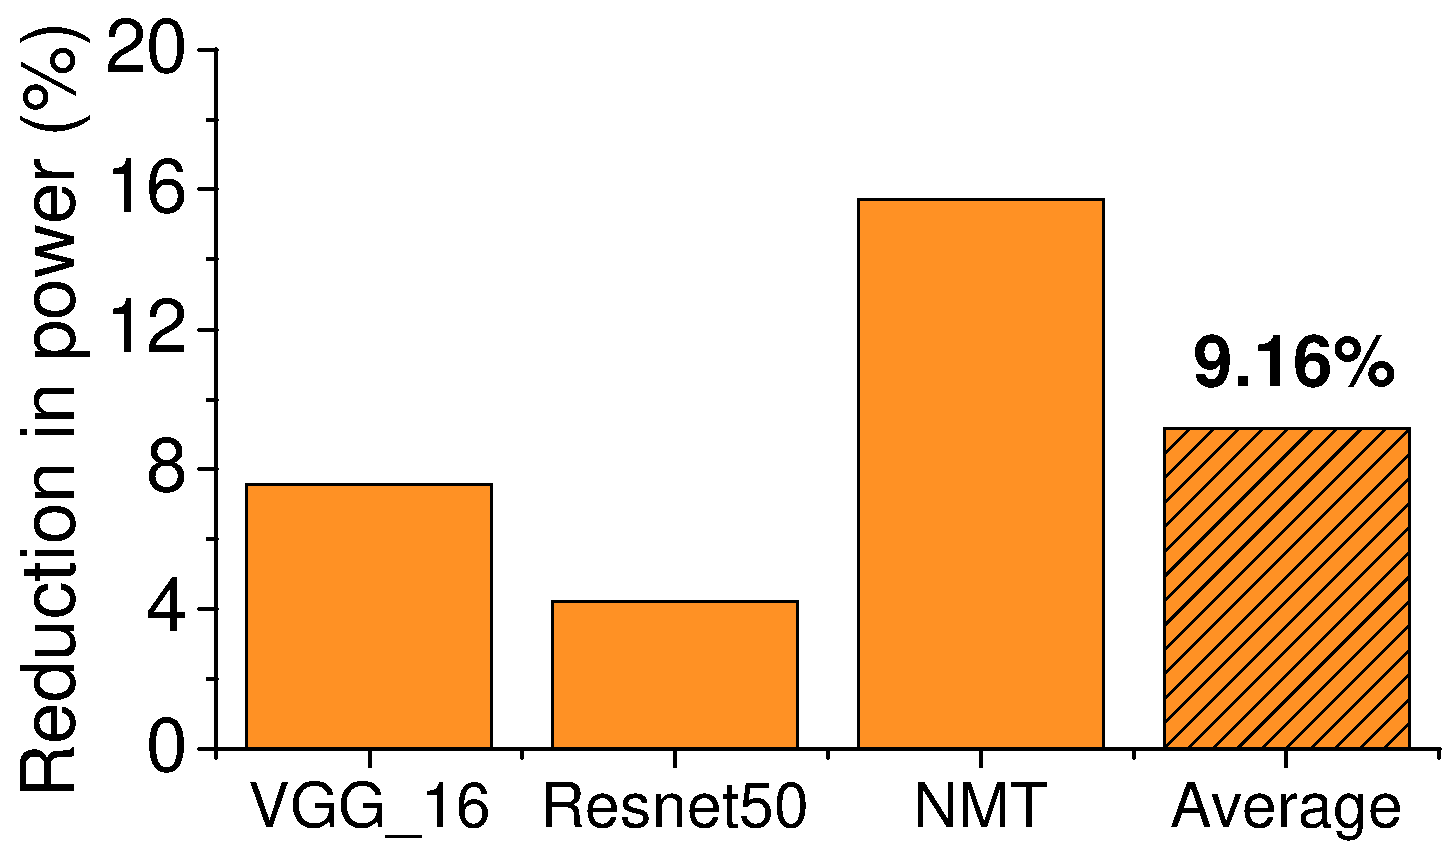
\includegraphics[width=0.3\textwidth]{figure/prun_power.pdf}}
\hfill
\subfloat[][Energy consumption]{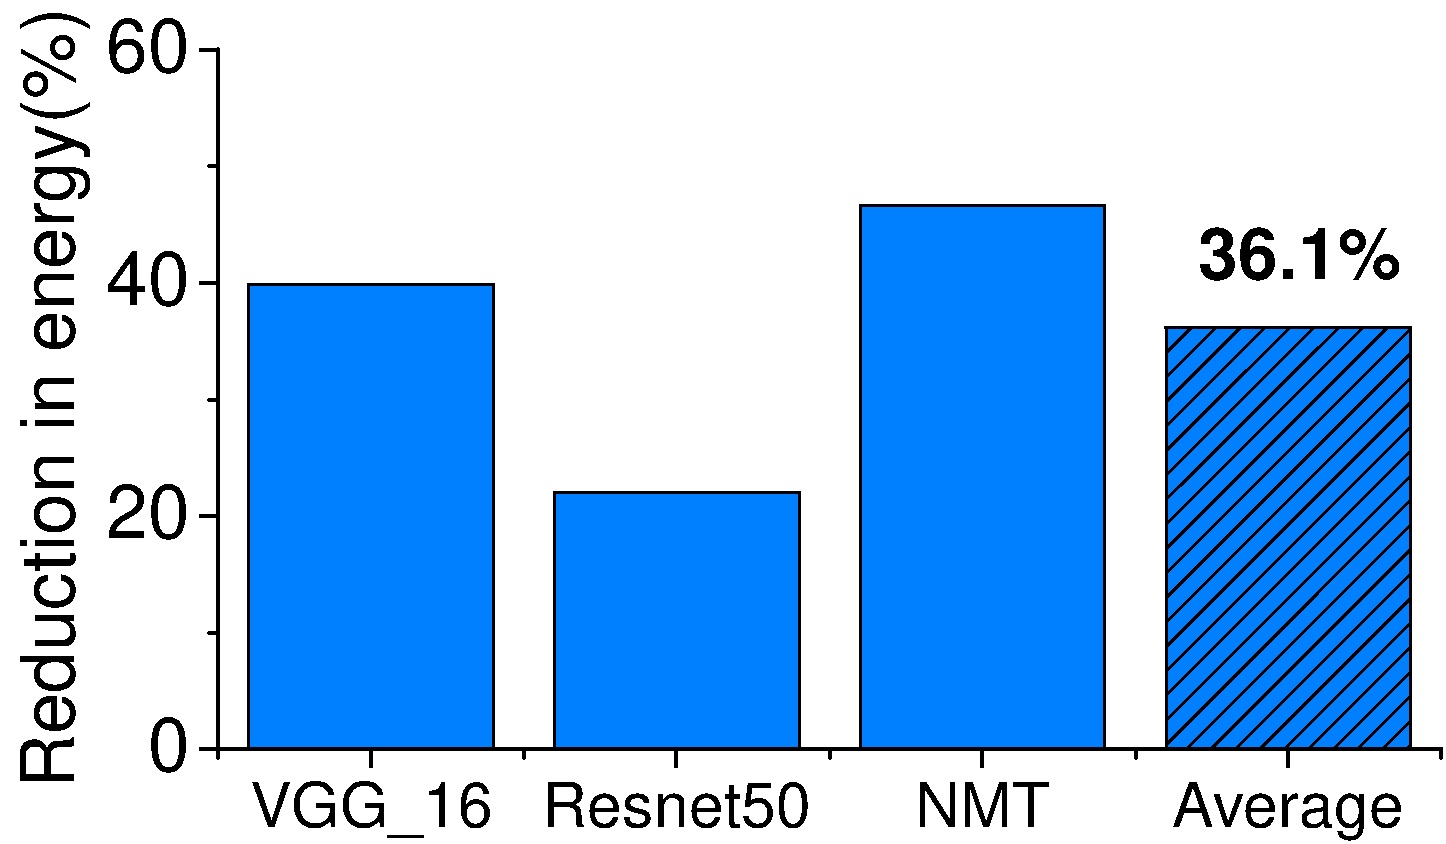
\includegraphics[width=0.3\textwidth]{figure/prun_energy.pdf}}
\hfill
\subfloat[][precision, recall and F1 score]{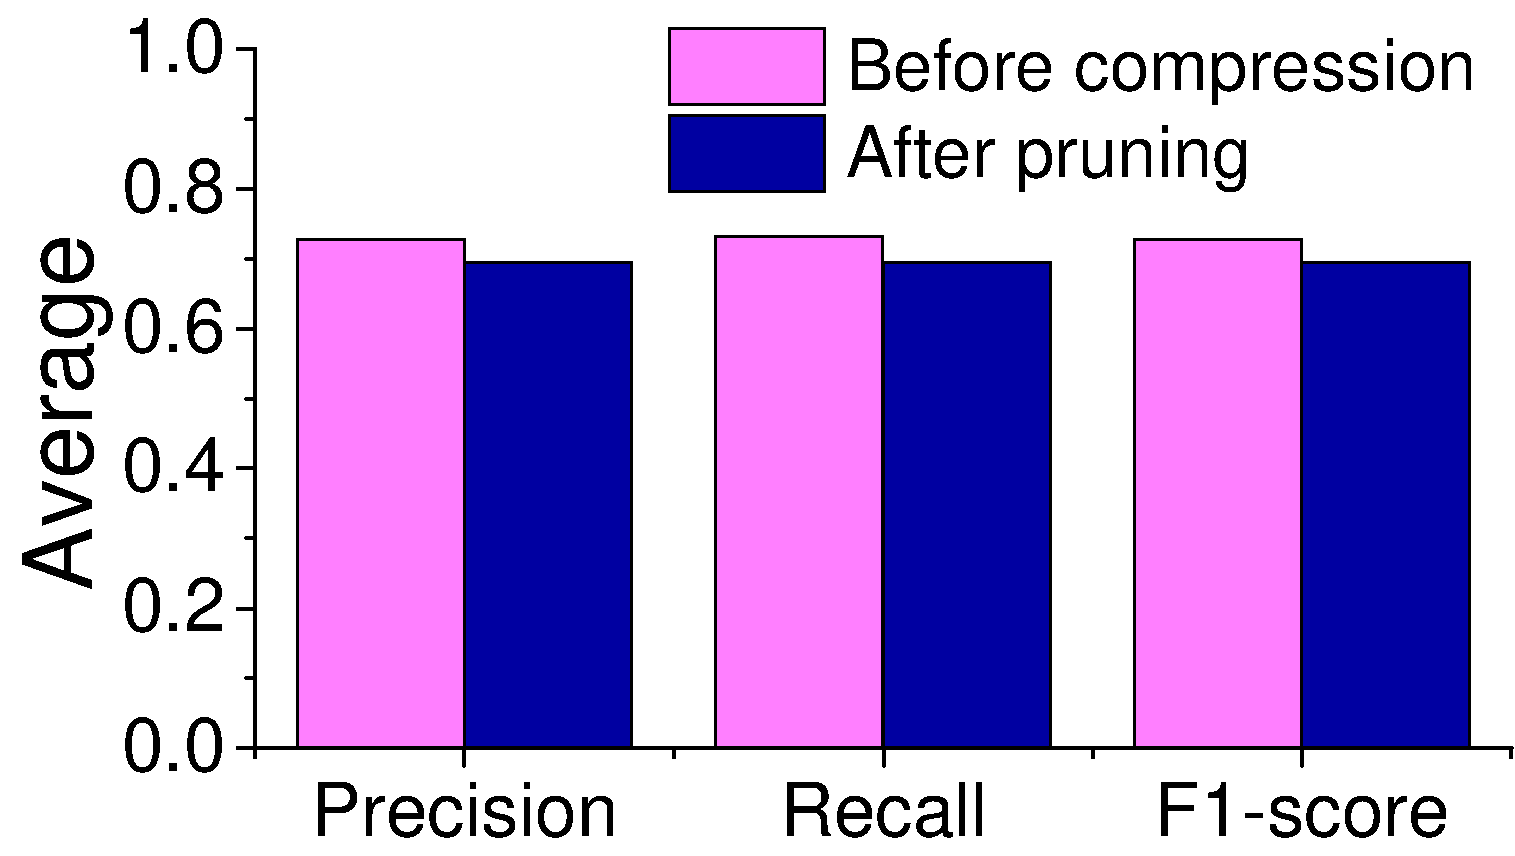
\includegraphics[width=0.3\textwidth]{figure/prun_prf.pdf}}
\hfill

\caption{The change of the model size (a), inference time (b), accuracy/BLEU (c), power (d), energy consumption (e), and accuracy (e)
before and after applying \pruning.} \label{fig:analy_prun}
\end{figure*}

\section{Experimental Results}


\subsection{Roadmap}
Our experiments try to answer the following questions:

\begin{itemize}
\item bla
\item bla2
\item bla3
\end{itemize}

\subsection{Impact on the Model Storage Size\label{sec:ms}}
Reducing the model storage size is crucial for embedded and IoT systems which often have a limited storage space. A smaller model size also
translates to smaller runtime memory footprint of less RAM space consumption. Figures~\ref{fig:analy_quan} and  \ref{fig:analy_prun}
illustrate how the different compression techniques and parameters affect the resulting model size.

As can be seen from Figure~\ref{fig:analy_quan}a, data quantization can significantly reduce the model storage size, leading to an average
reduction of 50.2\% when using a 16-bit representation and up to 80.7\% when using a 6-bit representation. The reduction in the storage
size is consistent across neural networks as the size of a network is dominated by its weights.

From Figure~\ref{fig:analy_prun}a, we see that by removing some of the pathways of the neural network, \pruning can also reduce the model
size, although the gain is smaller than \quantization. On average, \pruning reduces the model size by 27.2\% (49.26 MB). An interesting
observation is that, \pruning is particularly effective for obtaining a compact model for NMT, an \RNN, with a reduction of 60\% on the
model size. This is because there are typically many repetitive pathways in an \RNN due to the natural of the network architecture. As we
will discuss later, \pruning only leads to a minor degradation in the prediction accuracy for NMT. This suggests that \pruning can be an
effective model compression technique for \RNNs.



\subsection{Impact on Inference Time\label{sec:time}}
 Figure~\ref{fig:analy_quan}b compares the inference time when using different bit
widths to represent a 32-bit floating number for neural network weights. Intuitively, a smaller model should run faster. However, data
quantization does not reduce the inference time but instead it prolongs it. Data quantization can speedup the computation (i.e., matrix
multiplications) performed on the input data by avoiding expensive floating point arithmetics and enabling SIMD vectorization by using a
compact data representation. However, we found that the overhead of the quantization process during inference can outweigh its benefit.
Except the genernal inference operation, a data quantization and de-quantization function has to be added into the compressed model. The quantization function converts the 32-bit to quantized weights, after inference operation which
accounts for 50.9\%, the de-quantization quantized
weights back to a 32-bit representation on the output layer to recover the loss in precision. As can be seen from Figure~\ref{fig:breakdown}, this process could be expensive, contributing to 30\% to 50\% of the end to end inference time.
%this process could be expensive, contributing to 30\% to 50\% of the end to end inference time.
%After data quantization, a de-quantization function has to be added into the compressed model. This  function converts %the quantized
%weights back to a 32-bit representation on the output layer to recover the loss in precision. As can be seen from %Figure~\ref{fig:breakdown},
%this process could be expensive, contributing to 30\% to 50\% of the end to end inference time.

\begin{figure}
\begin{center}
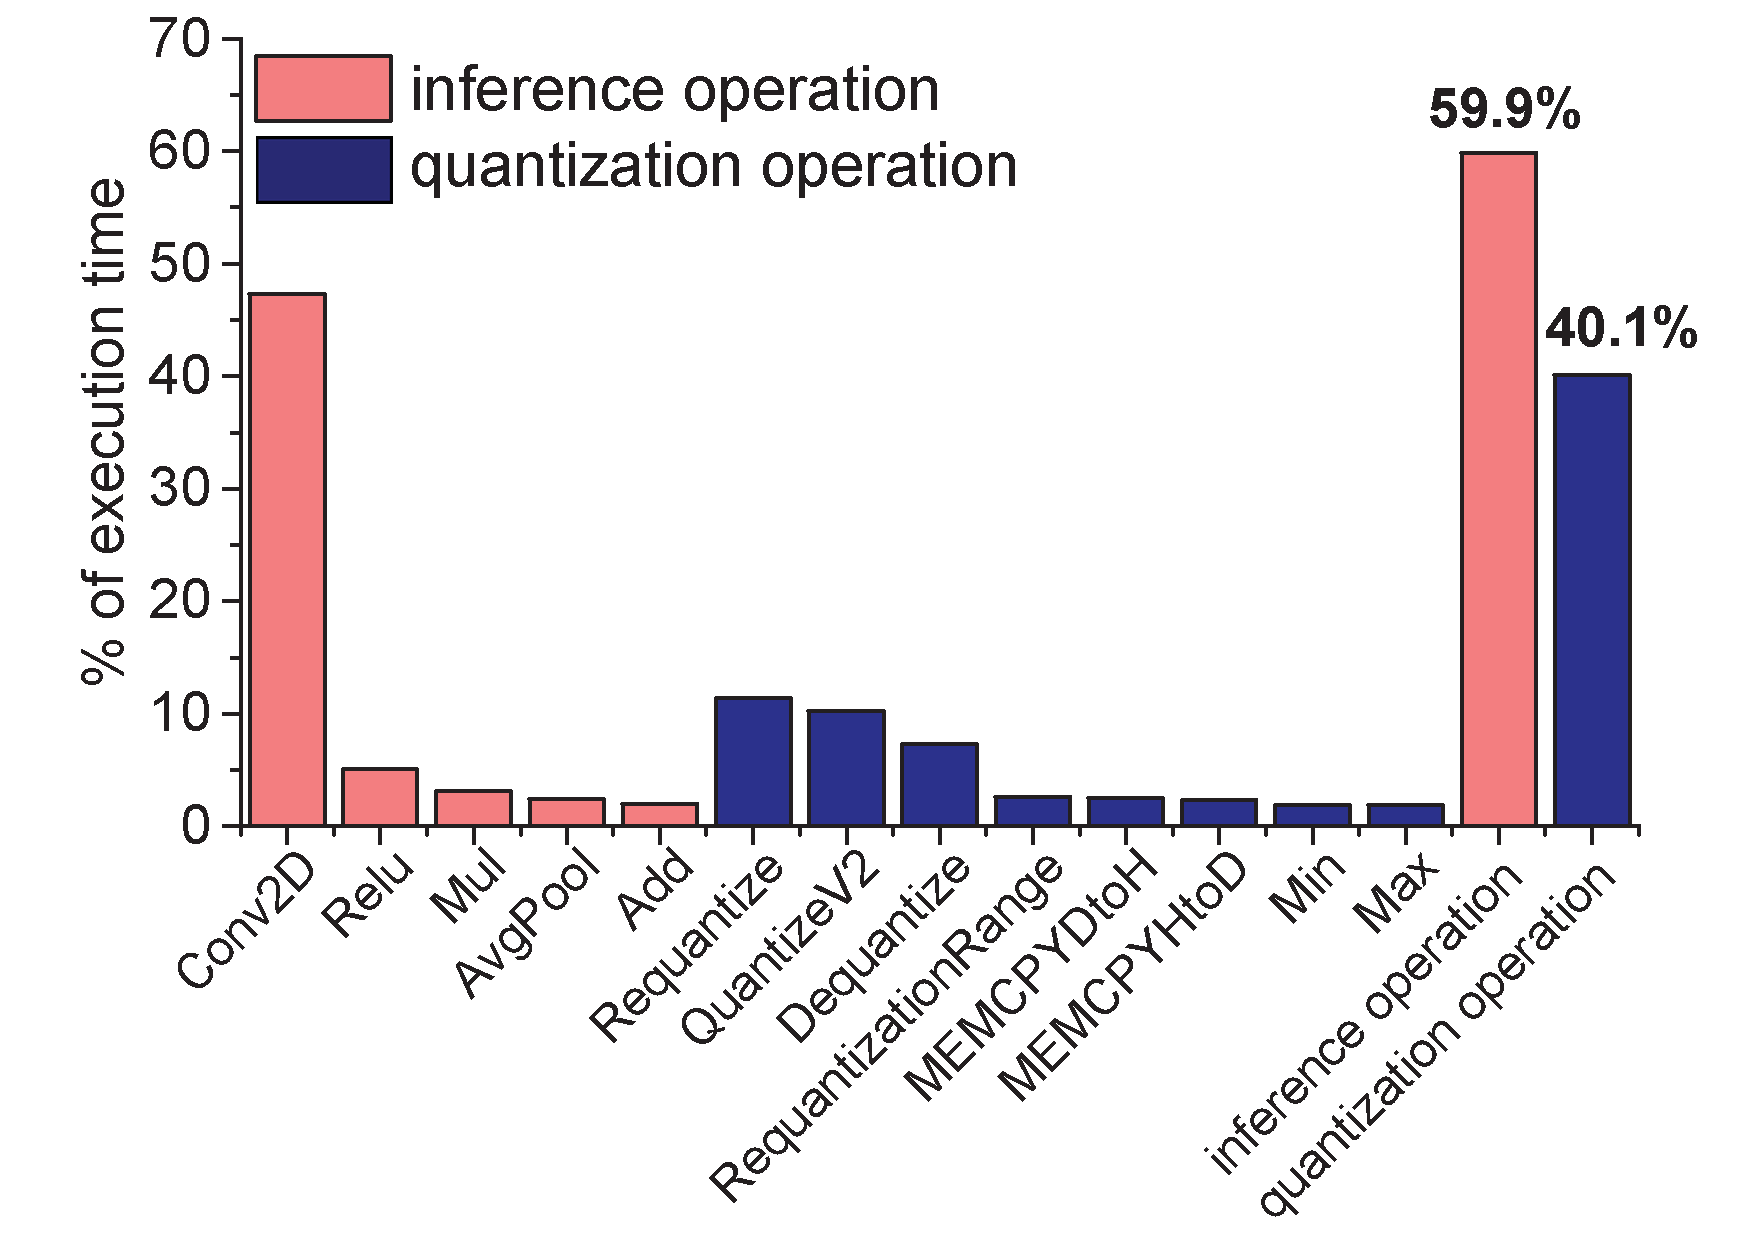
\includegraphics[width=0.48\textwidth]{figure/breakdown4.pdf}
\end{center}
\caption{Breakdown of the average execution time per operation type.}
\vspace{-2mm}
\label{fig:breakdown}
\end{figure}


Using fewer bits for representation can reduce the overhead of de-quantization. For example, using a 6-bit representation is 1.05x and
1.03x faster than using a 16-bit and a 8-bit representations, respectively. However, as we will demonstrate later when discussing
Figure~\ref{fig:analy_quan}c, using fewer bits has the drawback of causing larger degradation in the prediction accuracy. Hence, one must
carefully find a balance between the storage size, inference time, and prediction accuracy when applying data quantification.

We also find that the percentage of increased inference time depends on the neural network structure. Applying data quantization to
\texttt{Inception}, the most complex network in our \CNN tested set, will double the inference time. By contrast, data quantization only
leads to a 20\% increase in inference time for \texttt{Mobilenet}, a compact model. This observation suggests that data quantization may be
beneficial for simple neural networks on resource-constrained devices.


In contrast to \quantization, Figure~\ref{fig:analy_prun}b shows that \pruning leads to faster inference time across evaluated networks. We
can see that the inference time of \texttt{Vgg\_16} and \texttt{NMT} can benefit from this technique, with an reduction of 38\%.  Overall,
the average inference time is reduced by 31\%. This suggests that while \pruning is less effective in reducing the model size (see
Section~\ref{sec:ms}), it can be useful in achieving a faster inference time.


\subsection{Impact on Accuracy Metrics}
In addition to the storage size and inference time, accuracy is crucially important for a predictive model. A small and faster model is not
very useful if it gives wrong predictions all the time.


Results in Figure~\ref{fig:analy_quan}c compare how the prediction accuracy is affected by model compression. We see that the sweat spot of
\quantization depends on the neural network structure. An 16-bit representation keeps the most information of the original model and thus
leads to little reduction in the prediction accuracy, on average  1.36\%.  Using an 8-bit representation would lead on average 3.57\%
decrease in the accuracy, while using a 6-bit representation will lead to a significantly larger reduction of 10\% in  accuracy. We also
observe that some networks are more robust to \quantization. For example, while a 6-bit representation leads to less than 10\% decrease in
accuracy for \texttt{Resnet\_101}, it cause a 12\% drops in accuracy for \texttt{Resnet\_50}. This is because a more complex network (i.e.,
\texttt{Resnet\_101} in this case) is more resilient to the weight errors compared to network (i.e., \texttt{Resnet\_50} in this case) with
a smaller number of layers and neurons. Our findings suggest the need for having an adaptive scheme to choose the optimal \dquantization
parameter for given constraints.


For \pruning, the Figure~\ref{fig:analy_prun}c compares the reduction in the top-1 and the top-5 accuracies for \texttt{Vgg\_16} and
\texttt{Resnet\_50}. We also show the BLEU value for \texttt{NMT}. \pruning reduces the accuracy of the two \CNN models with by 5.7\% and
1.7\% respectively for the top-1 and top-5 scores. We observe that the \pruning has little negative impact on \texttt{NMT} where we only
observe an averaged loss of 0.8\% for BLEU. When taking into consideration that \pruning can significantly reduce the model size for
\texttt{NMT} (Section~\ref{sec:ms}), our results suggest that \pruning is particularly effective for \RNNs.


%Although an 8-bit representation leads to a minor
%decrease in the prediction accuracy, a further reduction of a 6-bit representation is only profitable for xx networks.



\subsection{Impact on the Power and Energy Consumption}
Power and energy consumption are two limiting factors on battery-powered mobile and IoT devices. As we can see from
Figure~\ref{fig:analy_prun}d, \quantization decreases the peak power for inferencing with an average of 4.3\%, 10.4\% and 11.6\%,
respectively when using a 6-bit, an 8-bit and a 16-bit representations. While \quantization reduces the peak power used, the increase
inference time leads to more energy consumption by at least 34.1\% and up to 51.1\% (see Figure~\ref{fig:analy_prun}e). This means that
although \quantization allows one to reduces voltage supply to the computing devices, it can lead to a short battery life.

Figure~\ref{fig:analy_prun}e shows the reduced energy consumption by applying \pruning. Note that it saves over 40\%, 15\% and 50\% energy
consumption for \texttt{Vgg\_16}, \texttt{Resne\_50} and \texttt{NMT} respectively. Despite that the peak power is reduced by only 9.16\%,
a smaller decrease compared to \quantization, the resulted faster inference time allows \pruning to significantly reduce the power
consumption. The results suggest \pruning is useful for reducing the overall energy consumption of the system, but \quantization can be
employed to support a low power system.



\subsection{Precision, Recall and F1-Score}

Finally, Figures~\ref{fig:analy_quan}f and \ref{fig:analy_prun}f show other three evaluation metrics of the considered deep learning models
after applying \quantization and \pruning. We can see that, the decrease in performance after compression is  less than 3\% for precision,
recall and F1-Score. For \quantization, the 16-bit representation outperforms the other two bits width representations. Specifically,
16-bit gives the highest overall precision, which in turns leads to the best F1 score. High precision can reduce false positive, which is
important for certain domains like video surveillance because it can reduce the human involvement for inspecting false positive
predictions.




\subsection{Memory footprint}

\begin{figure}[!t]
\centering
\subfloat[][\quantization]{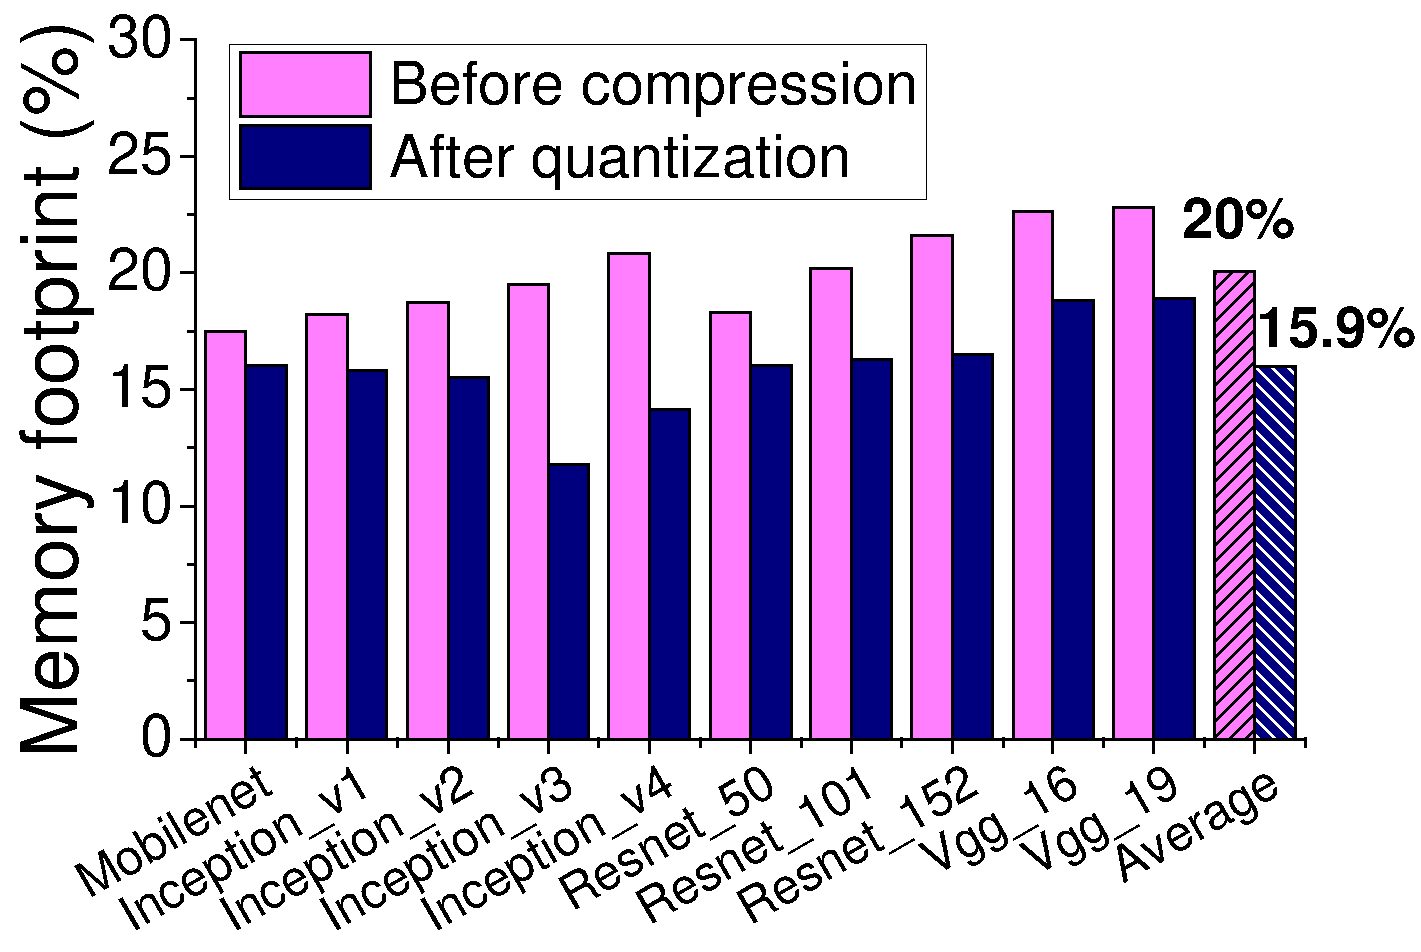
\includegraphics[width=0.4\textwidth]{figure/quan_mem.pdf}}
\hfill
\subfloat[][\pruning]{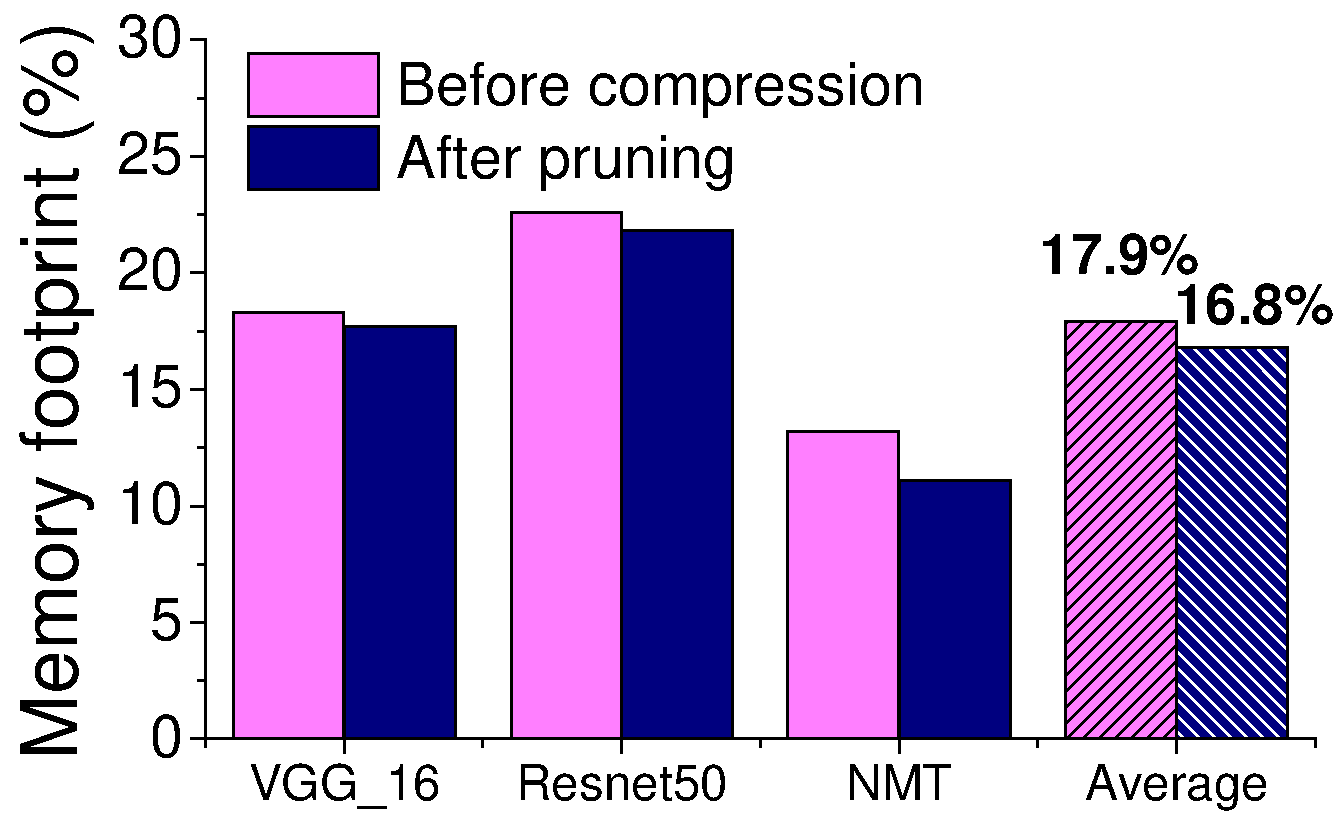
\includegraphics[width=0.4\textwidth]{figure/prun_mem.pdf}}
\hfill

\caption{Memory footprint before and after the compression by \quantization(a) and \pruning (b).}
\label{fig:footprint}
\end{figure}

Figure~\ref{fig:footprint} compares the resulting memory footprint by applying \quantization and \pruning. Quantization reduces the runtime
memory footprint with an averaged reduction of 17.2\% by generating a more compact model. For example, an 8-bit representation reduces the
memory footprint from 20.02\% to 15.97\% across networks, with an averaged reduction of 20.63\% (up to 40\%). In general, the smaller the
model storage size is, the less memory footprint the compressed model will be. As an example, a 6-bit representation uses \FIXME{xx, and
xx} less memory compared to a 8-bit and a 16-bit representations, respectively.

In contrast to \dquantization, Figure~\ref{fig:footprint} shows that  \pruning offers little help in reducing the model memory footprint.
On average, it leads to a 6.4\% reduction of memory footprint. This is because that the network weights still domain the memory resource
consumption, and \pruning is less effective compared to \dquantization for reducing the overhead of network weights.



\subsection{Compare to a Fixed Compression Setting}

\begin{figure}[!t]
\centering

\subfloat[][\quantization]{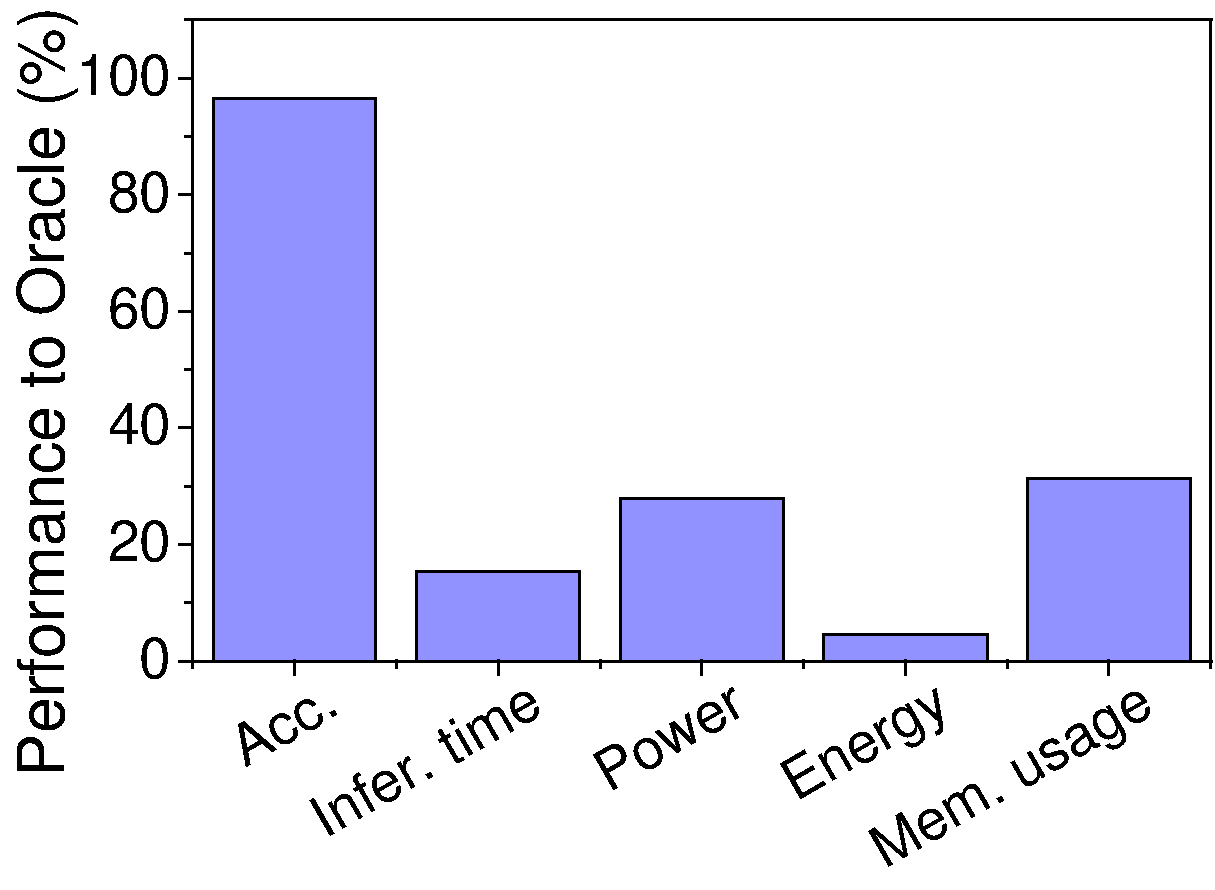
\includegraphics[width=0.35\textwidth]{figure/quan_oracle.pdf}}
\hfill
\subfloat[][\pruning]{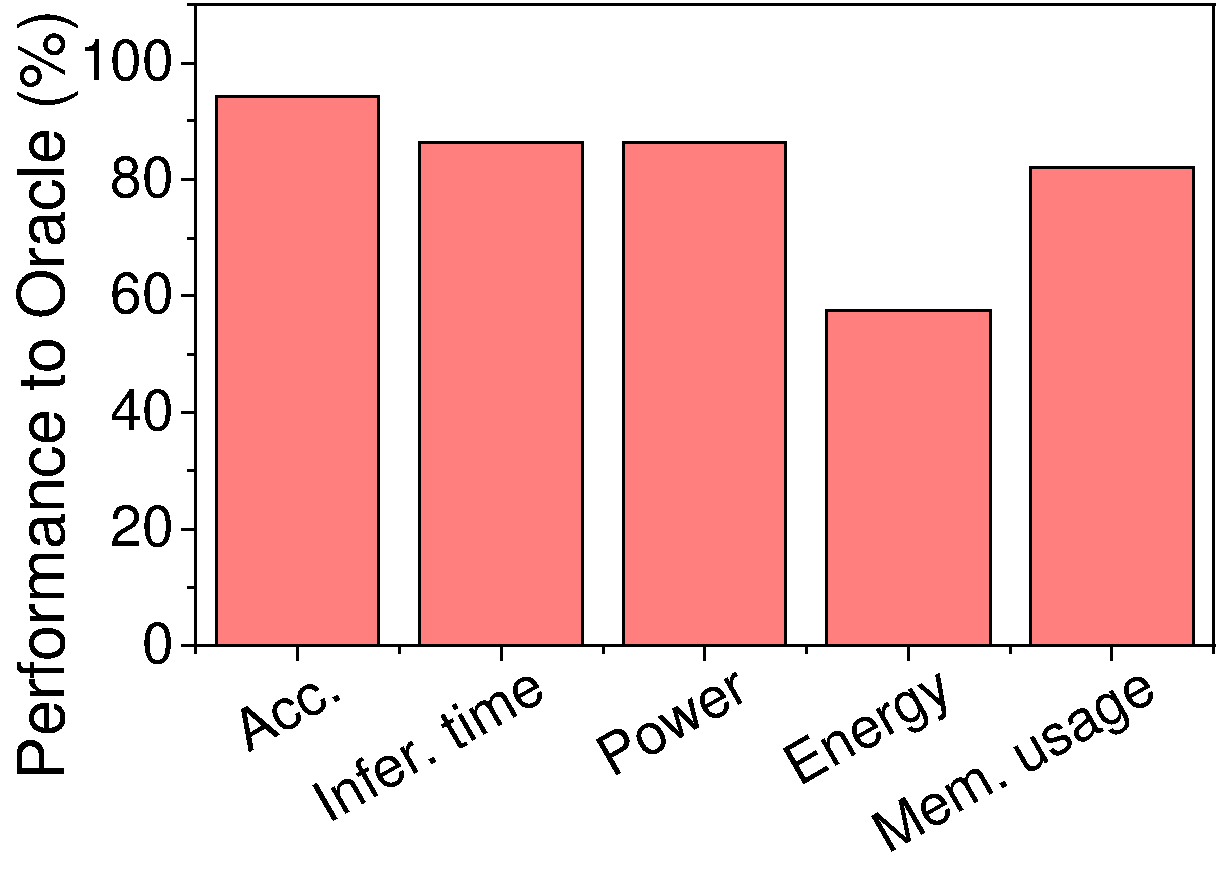
\includegraphics[width=0.35\textwidth]{figure/prun_oracle.pdf}}
\hfill

\caption{Compare to \FIXME{xx} for \quantization (a) and \pruning (b).} \label{fig:oracle}
\end{figure}

\FIXME{ZW: I have no idea of what's talking about here. Why a 8-bit data quantization setting is the oracle??? Please also use a spell
checker. }

In Figure~\ref{fig:oracle}, we compare our compressed models to ideal compressed models.
For \quantization, we use the 8-bit data quantization as the ideal
quantized weight, 
as it offers an affordable accuracy after quantization. 
We can see that,  the accuracy almost achieves the ideal value, on the
contary, the inference time and energy consumption perform worst, only account less than 10\%. Both of the inference time and memory usage
occupy more than 20\%. Figure~\ref{fig:oracle} b presents the how close our pruned models to the theoretically perfect models. As we can
see from this figure, most of evaluation metrics above 80\%, and the energy consumption also achieves 58\%.

\subsection{Combining Pruning and Quantization}

\begin{figure*}[!t]
\centering
\subfloat[][Model size]{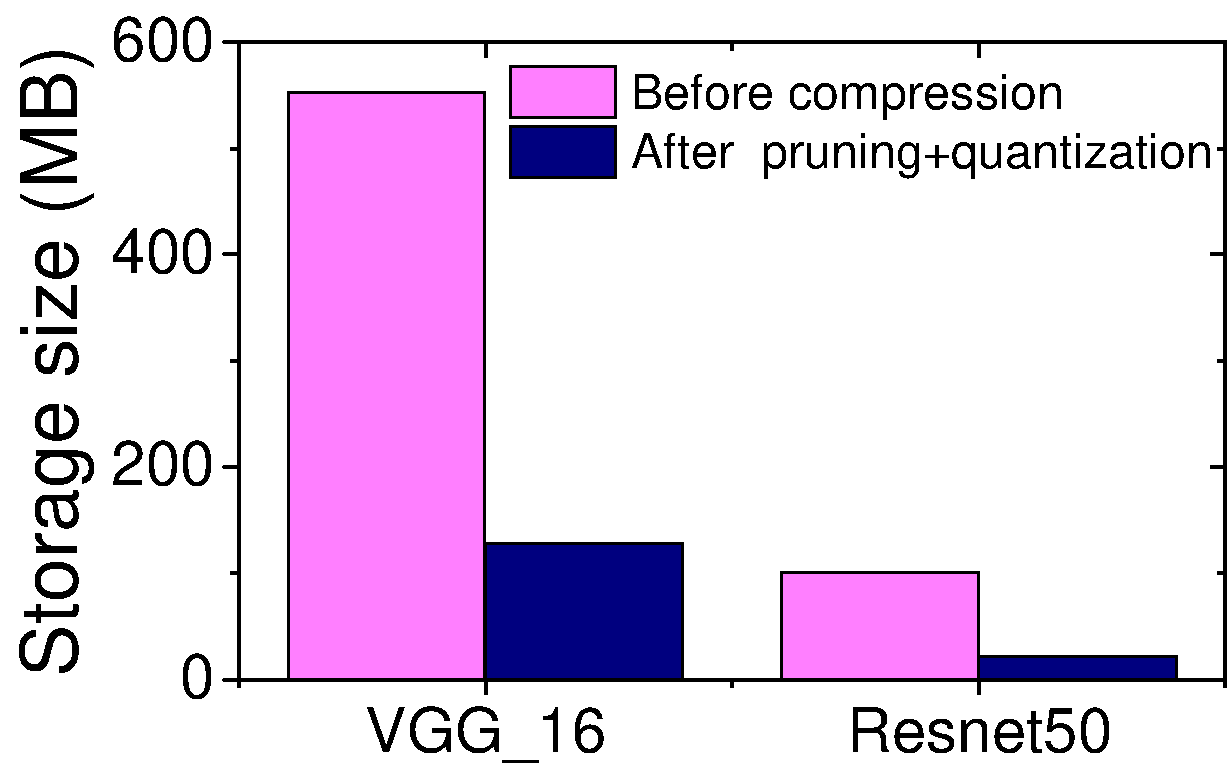
\includegraphics[width=0.24\textwidth]{figure/q_p_size.pdf}}
\hfill
\subfloat[][Inference time]{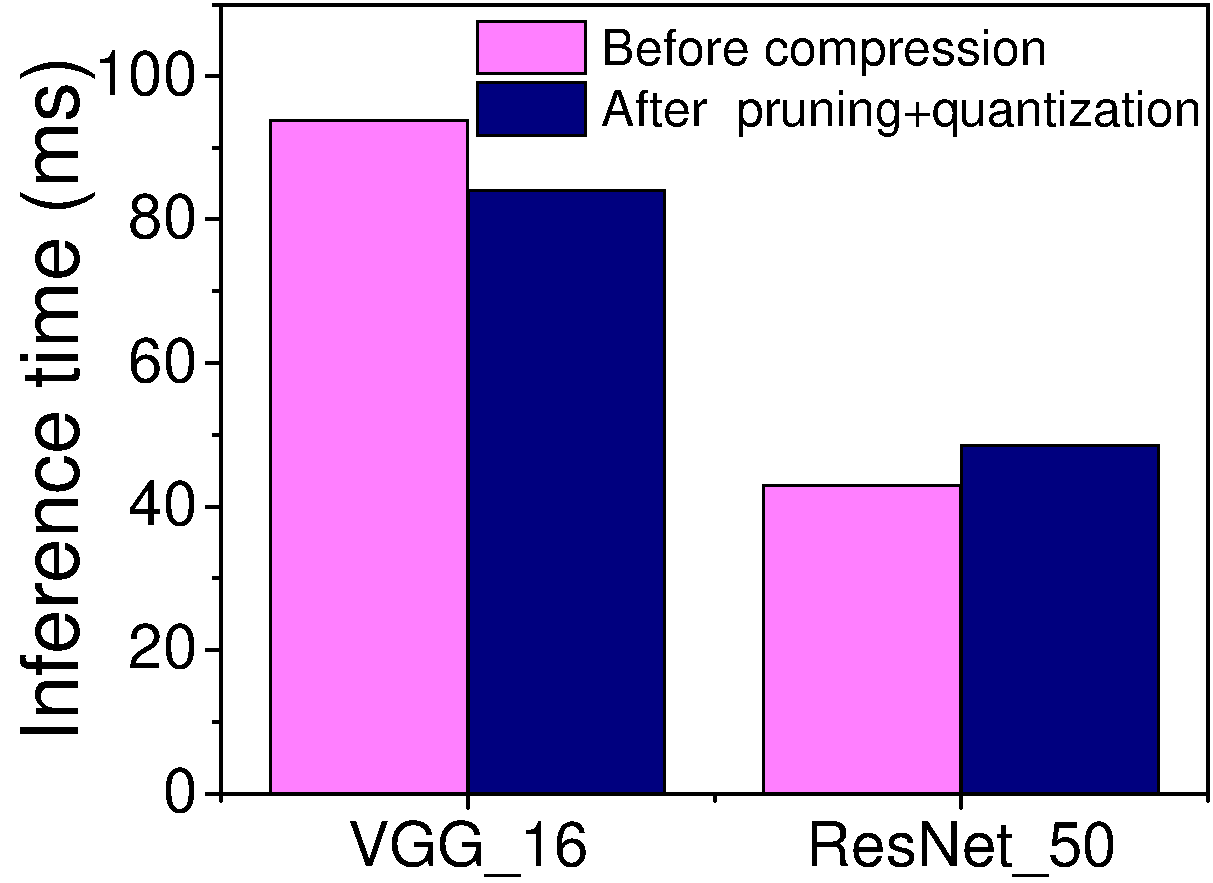
\includegraphics[width=0.24\textwidth]{figure/q_p_time.pdf}}
\hfill
\subfloat[][Energy consumption]{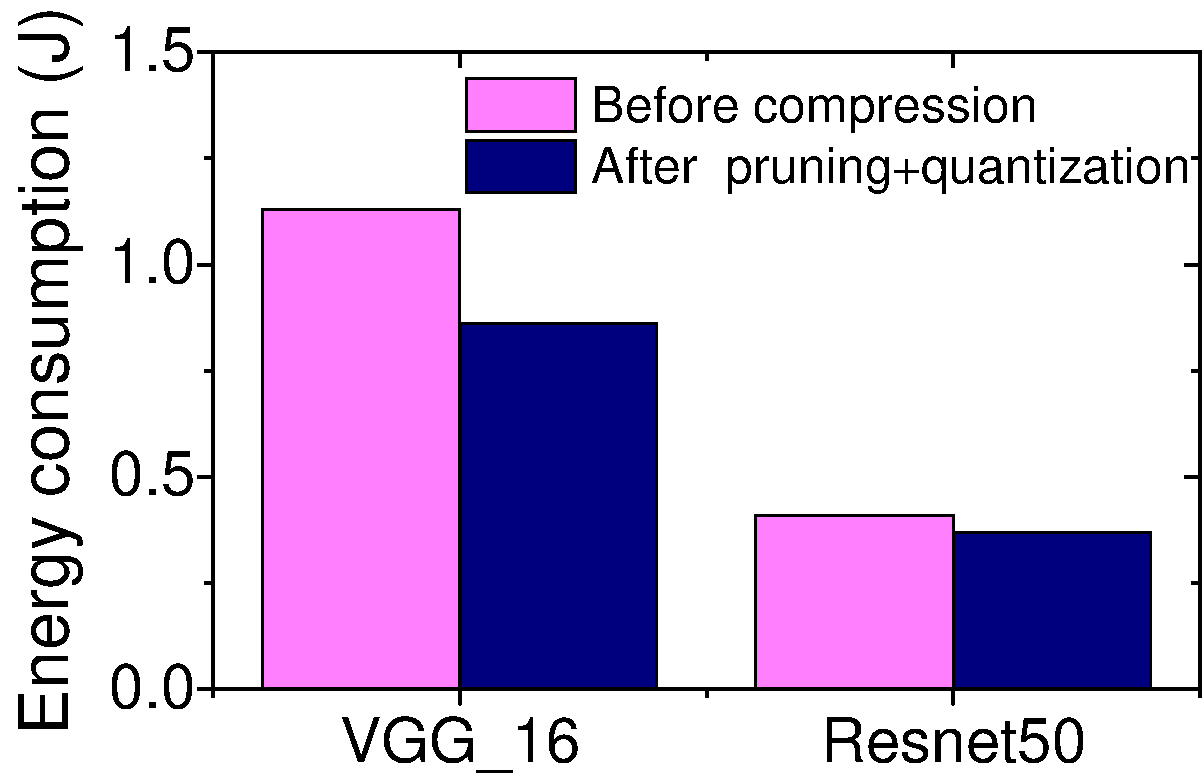
\includegraphics[width=0.23\textwidth]{figure/q_p_energy.pdf}}
\hfill
\subfloat[][Accuracy]{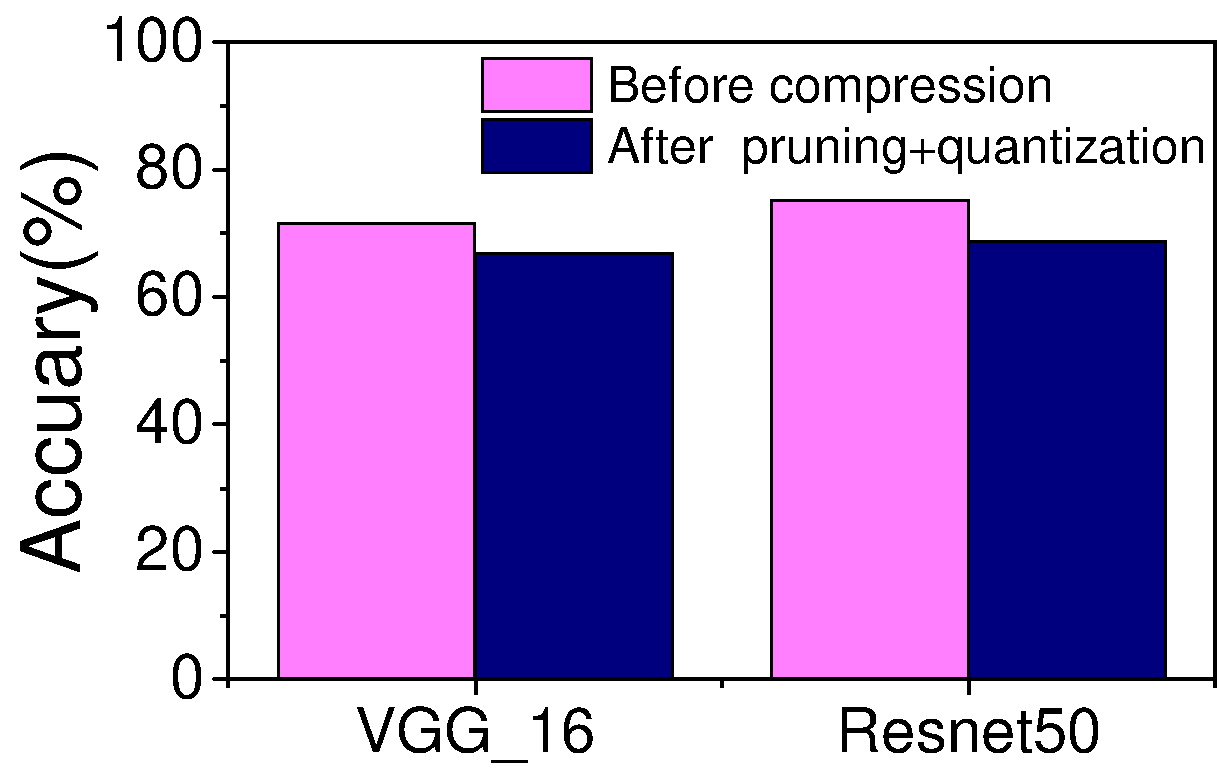
\includegraphics[width=0.24\textwidth]{figure/q_p_acc.pdf}}
\hfill
\caption{The achieved model size (a) inference time (b) energy consumption (c) and accuracy (d) before and after applying \quantization and \pruning.
}
\label{fig:combine}
\end{figure*}

So far we have evaluated \pruning and \quantization in isolation. An natural question to ask is: ``Is it worthwhile to combine both
techniques?". Figure~\ref{fig:combine} shows the results by first applying a 8-bit \dquantization and then \pruning to \texttt{VGG\_16} and
\texttt{Resnet50}.


As can be seen from Figure~\ref{fig:combine}a, combining both compression techniques can significantly reduce the model storage size -- the
resulting models are 76\% smaller than the original model. There is little degradation in the top-1 prediction accuracy
(Figure~\ref{fig:combine}d) -- less than 7\%. From Figure~\ref{fig:combine}b, we see that the combination has positive impact on the
inference time for \texttt{VGG\_16} as the runtime overhead of \dquantization (see Section~\ref{sec:time}) can be amortized by \pruning.
The combination, however, leads to longer inference time for \texttt{Resnet50} due to the expensive \dquantization overhead. Because of the
difference in inference time, there is less benefit in the energy reduction for \texttt{Resnet50} compared to what is obtained for
\texttt{VGG\_16} (Figure~\ref{fig:combine}c). This experiment shows that combining \pruning and \quantization can be beneficial, but it
depends on the neural network architecture and what to optimize for.
